%% ma: L12-B05-0008
%% lop: 12
%% chuong: 1
%% bai: 5
%% dang: 12.5.5
%% loai: TLN
%% muc: VDC
%% dap_an: "67,3"
%% nguon: "(NBV)-ĐỀ SỐ 6-MỖI NGÀY 1 ĐỀ THI 2025.pdf (D06, MỖI NGÀY 1 ĐỀ - Đề số 6), Phần III Câu 3 (Sở Ninh Bình 2025)"
%% kien_thuc: "Bài 5 (tối ưu hình học bằng đạo hàm); Bài 2 (GTLN của hàm số trên khoảng); phương trình đường tròn (lớp 10)"
%% trang_thai: chinh-thuc
%% ghi_chu: "Giáo viên đã duyệt 10/10/2026. Đáp án gốc 67,3 đúng (giá trị lớn nhất 67,3499... cm2, kiểm bằng sympy; sát ranh giới làm tròn nhưng vẫn là 67,3). Hình dựng lại bằng TikZ theo đề (kích thước tấm ván trên hình minh họa, không theo lời giải)"
\begin{ex}
Một thanh dầm hình hộp chữ nhật được cắt từ một khúc gỗ hình trụ có bán kính đáy bằng $20$ cm sao cho thanh dầm có diện tích mặt cắt ngang lớn nhất, tức là thanh dầm có mặt cắt ngang là hình vuông. Sau khi cắt thanh dầm đó, người ta lại cắt bốn tấm ván hình hộp chữ nhật từ bốn phần còn lại của khúc gỗ (tham khảo hình vẽ dưới). Xác định diện tích mặt cắt ngang tối đa của mỗi tấm ván (theo đơn vị $\text{cm}^2$ và làm tròn kết quả đến hàng phần chục).
\begin{center}
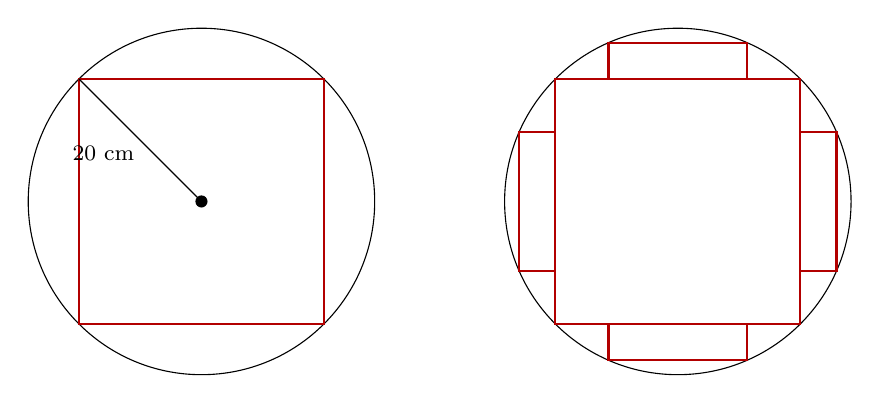
\begin{tikzpicture}[x=.11cm,y=.11cm]
  \def\q{14.142}\def\a{8}\def\t{18.33}
  \begin{scope}
    \draw (0,0) circle (20);
    \draw[red!70!black,thick] (-\q,-\q) rectangle (\q,\q);
    \fill (0,0) circle (.7);
    \draw (0,0)--(-\q,\q) node[midway,below left,font=\footnotesize,inner sep=2pt]{$20$ cm};
  \end{scope}
  \begin{scope}[shift={(55,0)}]
    \draw (0,0) circle (20);
    \draw[red!70!black,thick] (-\q,-\q) rectangle (\q,\q);
    \draw[red!70!black,thick] (-\a,\q) rectangle (\a,\t) (-\a,-\t) rectangle (\a,-\q)
                              (\q,-\a) rectangle (\t,\a) (-\t,-\a) rectangle (-\q,\a);
  \end{scope}
\end{tikzpicture}
\end{center}
\shortans{67,3}
\loigiai{Hình vuông nội tiếp đường tròn bán kính $20$ có đường chéo $40$, cạnh $20\sqrt2$. Chọn hệ trục $Oxy$ có $O$ là tâm đường tròn; phần gỗ còn lại phía trên cạnh $AB$ của hình vuông nằm dưới cung $y=\sqrt{400-x^2}$ và trên đường thẳng $y=10\sqrt2$.

Tấm ván có đỉnh $(a;\sqrt{400-a^2})$ trên đường tròn, $0<a<10\sqrt2$, nên diện tích mặt cắt ngang là $S(a)=2a\left(\sqrt{400-a^2}-10\sqrt2\right)$.

$S'(a)=0\Leftrightarrow a^2=175-\sqrt{10625}\approx71{,}9$, tức $a\approx8{,}48$. Lập bảng biến thiên (hoặc dùng máy tính) được $\max S=S(8{,}48)\approx67{,}35\ \text{cm}^2$, làm tròn đến hàng phần chục là $67{,}3$.}
\end{ex}
